\newpage
\appendix
\addcontentsline{toc}{section}{Appendices}
\section*{Appendices}
\section{Newtoniaanse bepaling afbuighoek als gevolg van een gravitationeel veld}
\label{appendix: newton}
Er wordt vertrokken vanuit de bewegingsvergelijkingen voor een deeltje in een potentiaal, gecreëerd door het zwaartekrachtveld. Er wordt aangetoond dat de oplossingen van de bewegingsvergelijking kegelsneden (cirkel, ellips, hyperbool, parabool) als oplossing heeft. Deze afleiding is gebasserd op het handboek Analytical Mechanics van Hand en Finch, \cite{hand-1998}.
\subsection{De baan van een deeltje in een zwaartekrachtveld zijn kegelsneden}
Voor gravitatie wordt de potentiële energie gegeven door
$$V(r)=-\frac{GmM}{r}$$
De effectieve potentiële energie is gegeven door
$$V_{eff}(r)=-\frac{k}{r}+\frac{l^{2}}{2\mu r^{2}}$$
Hierin is $k=GmM$.\\
$\mu$ is de gereduceerde massa, deze wordt gevonden uit $\frac{1}{\mu}=\frac{1}{M}+\frac{1}{m}$\\
De bewegingsvergelijking wordt dan gegeven door
$$\mu\ddot{r}=\frac{l^{2}}{\mu r^{3}}-\frac{k}{r^{2}}$$
Deze vergelijking is niet lineair. We voeren een nieuwe variabele in. Stel $u=\frac{1}{r}$ en $\dot{\phi}=\frac{l}{\mu r^{2}}$, dit volgt uit behoud van draaimoment. We weten dan dat
$$\mu r^{2}\dot{\phi}=l;\ \ \ \ \ \mu r^{2}d\phi=ldt;\ \ \ \ \ dt=\frac{\mu}{lu^{2}}d\phi$$
Dan geldt er dat
\begin{align}
\dot{r}&=\frac{d}{dt}r=\frac{d}{dt}\left(\frac{1}{u}\right) \nonumber \\
&=-\frac{1}{u^{2}}\frac{du}{dt} \nonumber \\
&=-\frac{1}{u^{2}}\frac{du}{d\phi}\frac{d\phi}{dt} \nonumber \\
&=-\frac{1}{u^{2}}\frac{lu^{2}}{\mu}\frac{du}{d\phi} \nonumber \\
&=-\frac{l}{\mu}\frac{du}{d\phi} \nonumber 
\end{align}
De 2de afgeleide is gegeven door
\begin{align}
\ddot{r}&=\frac{d}{dt}\left[-\frac{l}{\mu}\frac{du}{dt}\right] \nonumber \\
&=-\frac{l}{\mu}\frac{d}{d\phi}\left(\frac{du}{d\phi}\right)\frac{d\phi}{dt} \nonumber \\
&=-\frac{l}{\mu}\frac{lu^{2}}{\mu}\frac{d^{2}u}{d\phi^{2}} \nonumber 
\end{align}
Dan krijgen we als differentiaalvergelijking van de baan dat
$$\frac{d^{2}u}{d\phi^{2}}+u=\frac{k\mu}{l^{2}}$$
De oplossing van deze differentiaalvergelijking is gegeven door
$$u(\phi)=\frac{\mu k}{l^{2}}+A\cos(\phi)$$
We gaan nu overgaan op Cartesische coördinaten. Stel $p=\frac{l^{2}}{\mu k}$ en stel $\epsilon=pA\geq0$. Dan geldt er
$$pu=1+\epsilon\cos(\phi)$$
$$p=r+r\epsilon \cos(\phi)$$
$$(p-\epsilon x)^{2}=x^{2}+y^{2}$$
De energie is gegeven door
\begin{align}
    E&=\frac{1}{2}\mu(\dot{r}^{2}+r^{2}\dot{\phi}^{2})-\frac{k}{r}\nonumber \\
    &=\frac{\mu k^{2}}{2l^{2}}(\epsilon^{2}-1)
    \label{for: energie}
\end{align}
Merk op dat de energie afhankelijk is van $\epsilon$. 
\begin{itemize}
\item  $\epsilon=0$: we hebben een minimum van de energie. Er geldt
$$x^{2}+y^{2}=p^{2}$$
Dit is exact gelijk aan de vergelijking van een cirkel met als straal p. Deze straal is exact gelijk aan het minimum van $V_{eff}$. 
\item $\epsilon=1$, dan is de energie gelijk aan 0. De baan is dan gegeven door
$$p^{2}+x^{2}-2px=x^{2}+y^{2}$$
$$2px=p^{2}-y^{2}$$
$$x(y)=\frac{p^{2}-y^{2}}{2p}$$
Dit is de baan van een parabool
\item $0<\epsilon<1$, dit komt overeen met een energie die kleiner is dan 0. De baan is dan gegeven door
$$p^{2}+\epsilon^{2}x^{2}-2\epsilon px-x^{2}-y^{2}=0$$
$$\left(1-\epsilon^{2}\right)x^{2}+2\epsilon px+y^{2}-p^{2}=0$$
\begin{align}
    &\left(1-\epsilon^{2}\right)\left(x^{2}+\frac{2\epsilon px}{(1-\epsilon^{2})}+\frac{\epsilon^{2}p^{2}}{(1-\epsilon^{2})^{2}} \frac{\epsilon^{2}p^{2}}{(1-\epsilon^{2})^{2}}\right)\nonumber \\
    &+y^{2}-p^{2}=0    \nonumber
\end{align}
$$\left(1-\epsilon^{2}\right)\left(x+\frac{\epsilon p}{(1-\epsilon^{2})}\right)^{2}+y^{2}-\frac{\epsilon^{2}p^{2}}{(1-\epsilon^{2})}-p^{2}=0$$
$$\left(1-\epsilon^{2}\right)\left(x+\frac{\epsilon p}{(1-\epsilon^{2})}\right)^{2}+y^{2}=\frac{p^{2}}{(1-\epsilon^{2})}$$
Dit kunnen we ook nog schrijven als
$$\frac{(x-x_{c})^{2}}{a^{2}}+\frac{y^{2}}{b^{2}}=1$$
Met: \\
$x_{c}=\frac{-\epsilon p}{1-\epsilon^{2}}$ \\
$p=\frac{l^{2}}{\mu k}$\\
$\epsilon = pA$\\
$a=\frac{p}{1-\epsilon^{2}}$\\
$b=\frac{p}{\sqrt{1-\epsilon^{2}}}$\\
Dit komt overeen met de baan van een ellips
\item $\epsilon > 1$, dit komt overeen met een energie die groter is dan 0. 
$$\frac{(x-x_{c})^{2}}{a^{2}}-\frac{y^{2}}{b^{2}}=1$$
Dit is de baan van een hyperbool
\end{itemize}
\subsection{De bijhorende afbuighoek voor een hyperbolische baan}
De verandering in kinetische energie van het deeltje met massa $m$ en snelheid $v$ in de potentiaal (per eenheidsmassa) is gegeven door 
\begin{equation}
    E=\frac{1}{2}mv^{2}
    \label{for:energie}
\end{equation}
Het draaimoment per eenheidsmassa is gegeven door
\begin{equation}
    L=bv
    \label{for:draaimoment}
\end{equation}
Deze twee grootheden kunnen ook geschreven worden in termen van de excentriciteit. Vertrekende van de energie gevonden in \cref{for: energie}, en gebruikmakende van $p=\frac{l^{2}}{\mu k}$ vinden we
$$E=\frac{k}{2p}(\epsilon^{2}-1)$$
We definiëren nu a als
$$a=\frac{p}{\epsilon^{2}-1}$$
Zo vinden we dan voor de energie per eenheidsmassa dat
\begin{align}
    E &= \frac{k}{2ma}\nonumber \\
    &= \frac{GM}{2a}
    \label{for:E}
\end{align}
Voor het draaimoment per eenheidsmassa geldt
\begin{align}
    L^{2} &= r^{2}v^{2}\nonumber \\
    &= r^{2}\cdot 2E \nonumber \\
    &= \frac{GM}{a}\cdot b^{2}
    \label{for:L2}
\end{align}
\begin{figure}
    \centering
    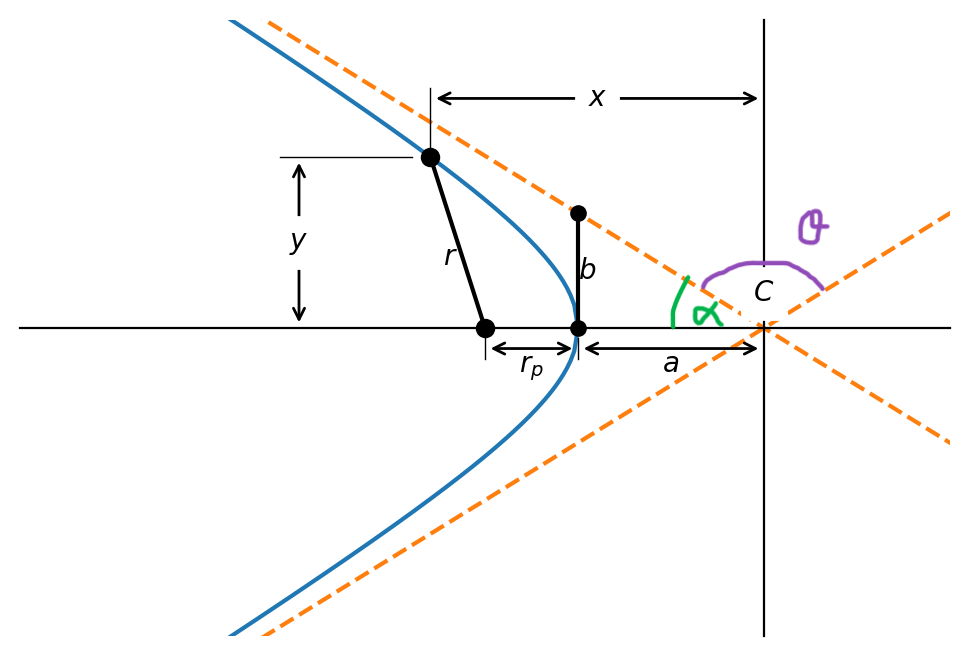
\includegraphics[width=0.95\linewidth]{Figures/hoek_hyperbool.png}
    \caption{De halve hoek van een hyperbolische baan. Figuur van Weber, \cite{weber-no-date}}
    \label{fig: halve hoek}
\end{figure}
De halve hoek van de hyperbolische baan is te zien in \cref{fig: halve hoek}. Daaruit volgt eenvoudig dat:
\begin{equation}
    tan(\alpha) = \frac{b}{a}
    \label{for: hoek}
\end{equation}
We gaan \cref{for: hoek} herschrijven in termen van L (\cref{for:L2}) en E (\cref{for:E}).
Merk op dat
$$E\cdot L^{2}=\frac{G^{2}M^{2}b^{2}}{2a^{2}}$$
$$\frac{2E\cdot L^{2}}{G^{2}M^{2}}=\frac{b^{2}}{a^{2}}$$
$$\frac{\sqrt{2E}L}{GM}=\frac{b}{a}$$
Invullen van \cref{for:energie} en \cref{for:draaimoment} geeft
\begin{align}
    \frac{b}{a}&=\frac{\sqrt{2\cdot\frac{1}{2}v^{2}}rv}{GM}\nonumber \\
     &= \frac{rv^{2}}{GM}\nonumber\\
\end{align}
Voor de hoek vinden we dan
\begin{equation}
    \tan(\alpha) =\frac{rv^{2}}{GM} 
    \label{for:tangens}
\end{equation}
De afbuighoek is gegeven door de hoek tussen de asymptoten. Als we kijken op \cref{fig: halve hoek} dan zien we
$$\theta = \pi - 2\alpha$$
Omvormen naar $\alpha$ geeft
$$\alpha = \frac{\pi}{2}-\frac{\theta}{2}$$
De tangens nemen
\begin{equation}
    \tan(\alpha) = \tan\left(\frac{\pi}{2}-\frac{\theta}{2}\right)
    \label{for:tan}
\end{equation}
We herschrijven de laatste tangens:
\begin{align}
    \tan\left(\frac{\pi}{2}-\frac{\theta}{2}\right)&=\frac{\sin(\frac{\pi}{2}-\frac{\theta}{2})}{\cos(\frac{\pi}{2}-\frac{\theta}{2})}\nonumber\\
    &= \frac{\cos(\frac{\theta}{2})}{\sin(\frac{\theta}{2})}\nonumber \\
    & = \cot(\frac{\theta}{2})
    \label{for:cot}
\end{align}
Invullen van \cref{for:cot} in \cref{for:tan} geeft
\begin{equation}
    tan(\alpha) = \frac{1}{tan(\frac{\theta}{2})}
    \label{for:afbuighoek}
\end{equation}
Invullen van \cref{for:tangens} en Taylor toepassen voor kleine $\theta$
$$\frac{1}{tan(\frac{\theta}{2})} = \frac{rv^{2}}{GM}$$
$$\frac{1}{\frac{\theta}{2}}=\frac{rv^{2}}{GM}$$
$$\frac{\theta}{2} = \frac{GM}{rv^{2}}$$
$$\theta = \frac{2GM}{rv^{2}}$$
Als de afbuiging van licht beschouwd wordt is de snelheid gegeven door de snelheid van het licht. Dan is de afbuighoek gegeven door \cref{for: afbuighoek}.
\begin{equation}
    \theta = \frac{2GM}{rc^{2}}
    \label{for: afbuighoek}
\end{equation}
Dit was nu de afleiding voor de hyperbool. Merk op dat dit de Newtoniaanse afleiding was. Als de gravitationele correcties mee in rekening gebracht worden, wordt in de teller een extra factor 2 gevonden.
\section{De lensvergelijking}
\label{appendix:lensvergelijking}
De werking van de lens kan benaderd worden als een geometrisch probleem in twee dimensies. De voorstelling van de werking van de lens is te zien in \cref{fig:lensvgl}
\begin{figure}[H]
    \centering
    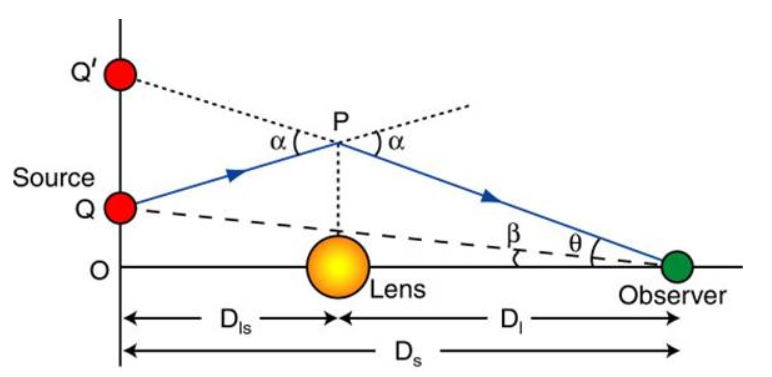
\includegraphics[scale=0.5]{Figures/Lensvergelijking.png}
    \caption{Schets van de werking van de lens in twee dimensies. Figuur van Jodrell Bank Centre for astrophysics, \cite{jodrell-bank-centre-for-astrophysics-no-date}.}
    \label{fig:lensvgl}
\end{figure}\mbox{}
Om de lensvergelijking af te leiden wordt er gezocht naar de afstanden $OQ$, $OQ'$ en $QQ'$. Er wordt steeds aangenomen dat de hoeken klein zijn. Uit de figuur volgt er dat
$$\tan(\beta) = \frac{|OQ|}{D_{s}}$$
$$|OQ| = D_{s}\tan(\beta)$$
Doordat de hoeken klein zijn kunnen we Taylor rond $\beta=0$ toepassen. Er word dan gevonden dat
\begin{equation}
  |OQ| = D_{s}\beta  
  \label{for:OQ}
\end{equation}
Analoog voor $|OQ'|$ geldt er
\begin{equation}
   |OQ'| = D_{s}\theta 
   \label{for:OQ'}
\end{equation}
Om de afstand $|QQ'|$ te bepalen wordt er gewerkt in de driehoek $\Delta PQQ'$. Een close-up van de driehoek is te zien in \cref{fig:driehoek}.
\begin{figure}[h]
    \centering
    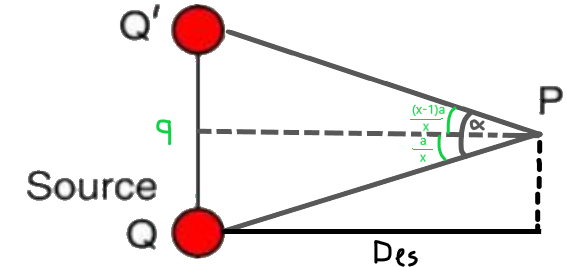
\includegraphics[scale=0.45]{Figures/driehoek.png}
    \caption{Close-up van de desbetreffende driehoek}
    \label{fig:driehoek}
\end{figure}
Er wordt opgemerkt dat $|QQ'| = |Qq|+|qQ'|$. Die twee afstanden zijn makkelijk te vinden uit de tangens. De hoek $\alpha$ wordt gesplitst in twee hoeken (die optellen tot $\alpha$). Zo wordt een rechthoekige driehoek verkregen. De eerste hoek is dan $\frac{\alpha}{x}$. De tweede hoek is gegeven door $\frac{(x-1)\alpha}{x}$. Zo zijn de twee afstanden gegeven door
$$\tan\left(\frac{\alpha}{x}\right)=\frac{|Qq|}{D_{ls}}$$
$$|Qq|=\tan\left(\frac{\alpha}{x}\right)D_{ls}$$
Analoog wordt er gevonden
$$\tan\left(\frac{(x-1)\alpha}{x}\right)=\frac{|qQ'|}{D_{ls}}$$
$$|qQ'|=\tan\left(\frac{(x-1)\alpha}{x}\right)D_{ls}$$
De som is dan gegeven door
$$|QQ'|=D_{ls}\left(\tan\left(\frac{\alpha}{x}\right)+\tan\left(\frac{(x-1)\alpha}{x}\right)\right)$$
Doordat de hoek $\alpha$ klein is kan er Taylor toegepast worden op de tangens, rond 0. Dan wordt er gevonden dat
\begin{align}
    |QQ'| &=D_{ls}\left(\frac{\alpha}{x}+\frac{x\alpha}{x}-\frac{\alpha}{x}\right) \nonumber\\
    &=D_{ls}\alpha
    \label{for:QQ'}
\end{align}
Nu de afstanden $|OQ|, |OQ'|$ en $|QQ'|$ gekend zijn (zie \cref{for:OQ}, \cref{for:OQ'} en \cref{for:QQ'}), kan de lensvergelijking gevonden worden. Het is eenvoudig in te zien dat $|OQ'|=|OQ|+|QQ'|$. Daaruit volgt
\begin{align}
    D_{s}\theta &=D_{s}\beta + D_{ls}\alpha \nonumber\\
    \theta &= \beta + \frac{D_{ls}}{D_{s}}\alpha \nonumber\\
    \beta &= \theta - \frac{D_{ls}}{D_{s}}\alpha
    \label{for: lensvgl}
\end{align}
\cref{for: lensvgl} wordt de lensvergelijking in 1D genoemd.
\onecolumn
\mbox{}
\section{Opbouw afschatten parameters van een sersic}
Voor de afschatting van de parameters van deze appendix werden 7\_500\_000 samples gegenereeerd, waarvan er 10\_500\_000 weggegooid werden.
\label{appendix: opbouw}
\begin{figure}[H]
    \begin{minipage}{0.95\textwidth}
        \centering
        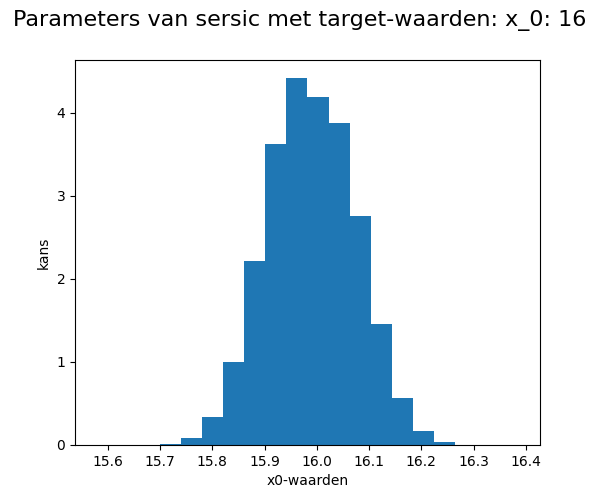
\includegraphics[width=0.3\textwidth]{Figures/1_sersic_verschillende_parameters/sersic_parameters_metropolis_7500000_1500000_10_x0_0.png}
        \subcaption[width=0.3\textwidth]{1 onbekende parameter}
        \centering
        \vspace{1cm}
        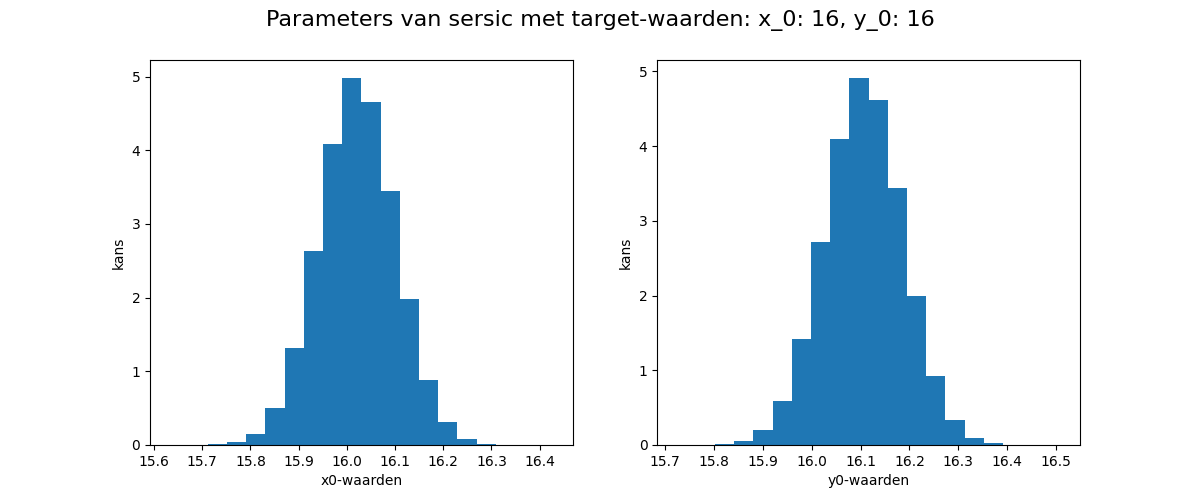
\includegraphics[width=0.60\textwidth]{Figures/1_sersic_verschillende_parameters/sersic_parameters_metropolis_7500000_1500000_10_y0_0.png}
        \subcaption[width=0.6\textwidth]{2 onbekende parameters}    
        \centering
        \vspace{1cm}
        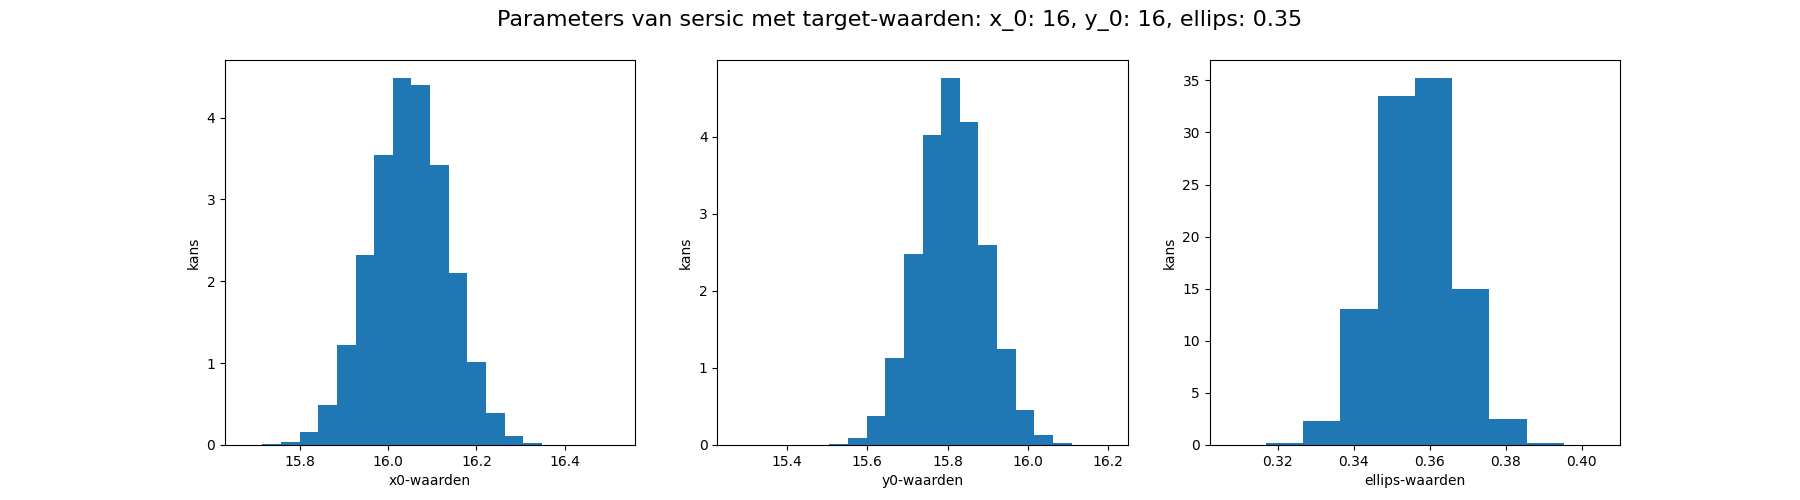
\includegraphics[width=0.93\textwidth]{Figures/1_sersic_verschillende_parameters/sersic_parameters_metropolis_7500000_1500000_10_ellips_0.png}
        \subcaption{3 onbekende parameters}
    \end{minipage}
    \caption{Het proces waarin telkens meer onbekende toegevoegd worden. Er wordt begonnen met één ongekende parameter, en toegewerkt naar drie onbekenden.}
    \label{fig:1 onbekende}
\end{figure}
\begin{figure}
    \begin{minipage}{0.95\textwidth}        
        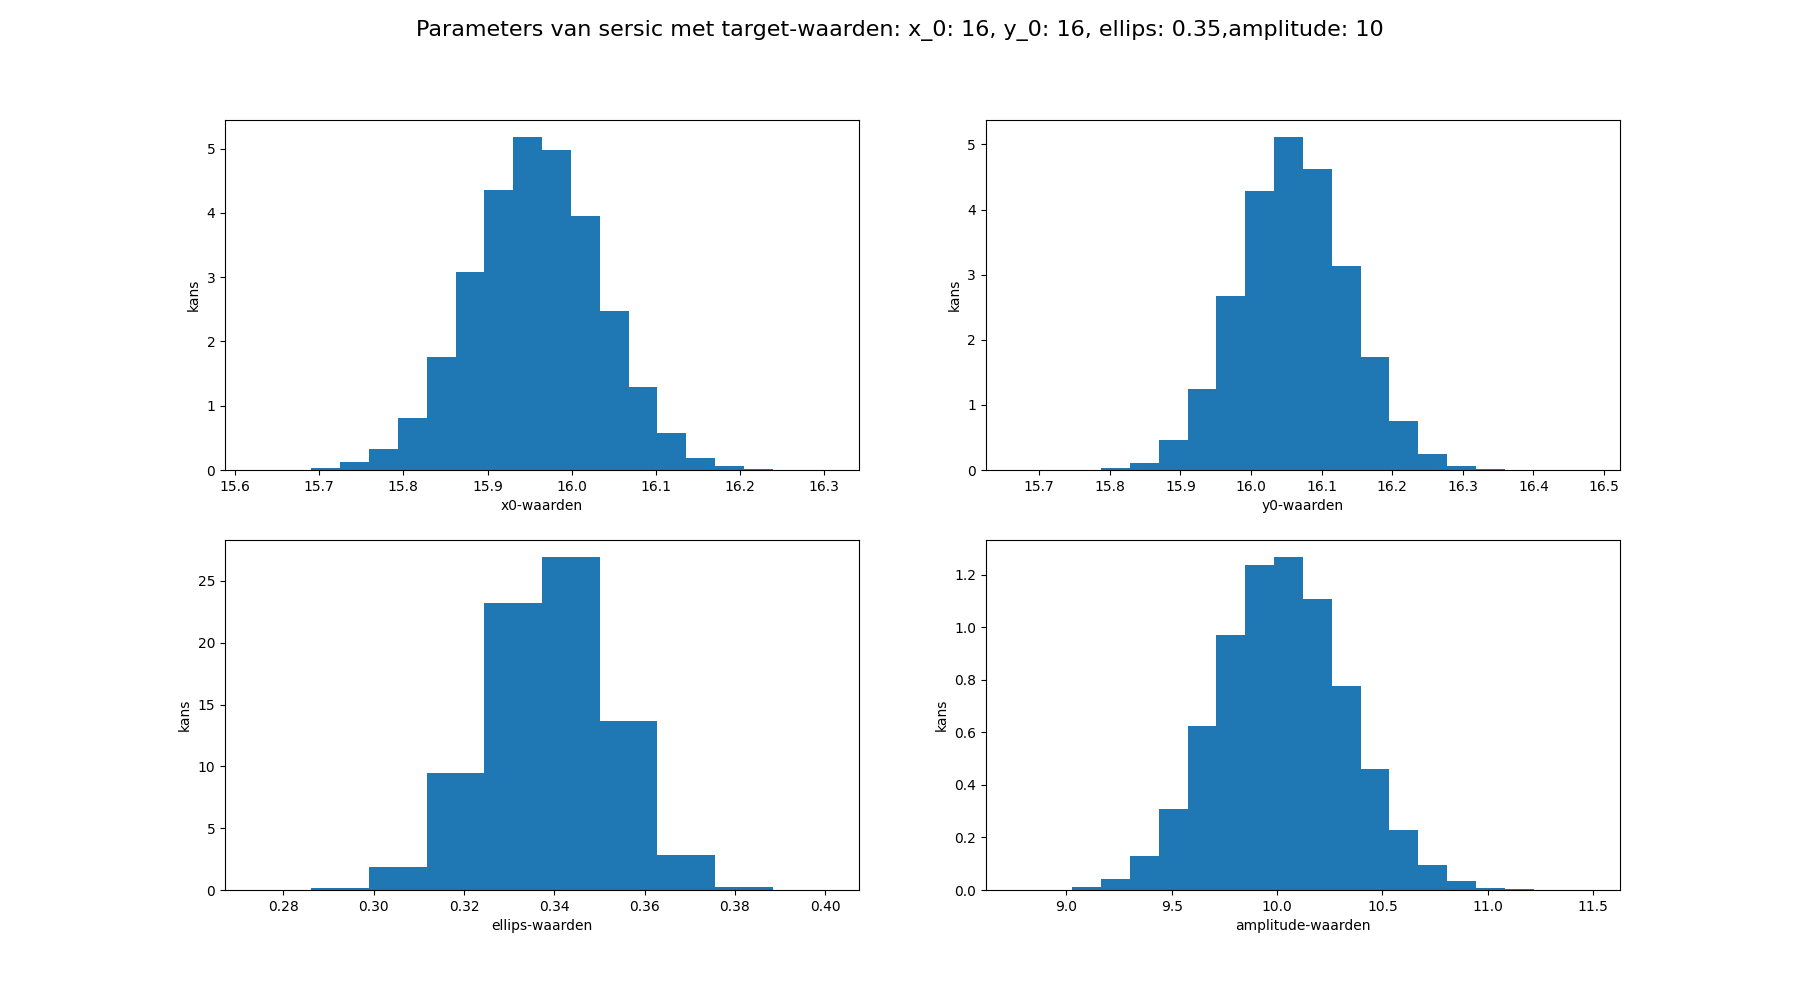
\includegraphics[width=0.93\textwidth]{Figures/1_sersic_verschillende_parameters/sersic_parameters_metropolis_7500000_1500000_10_amplitude_0.png}
        \subcaption{4 onbekende parameters}
        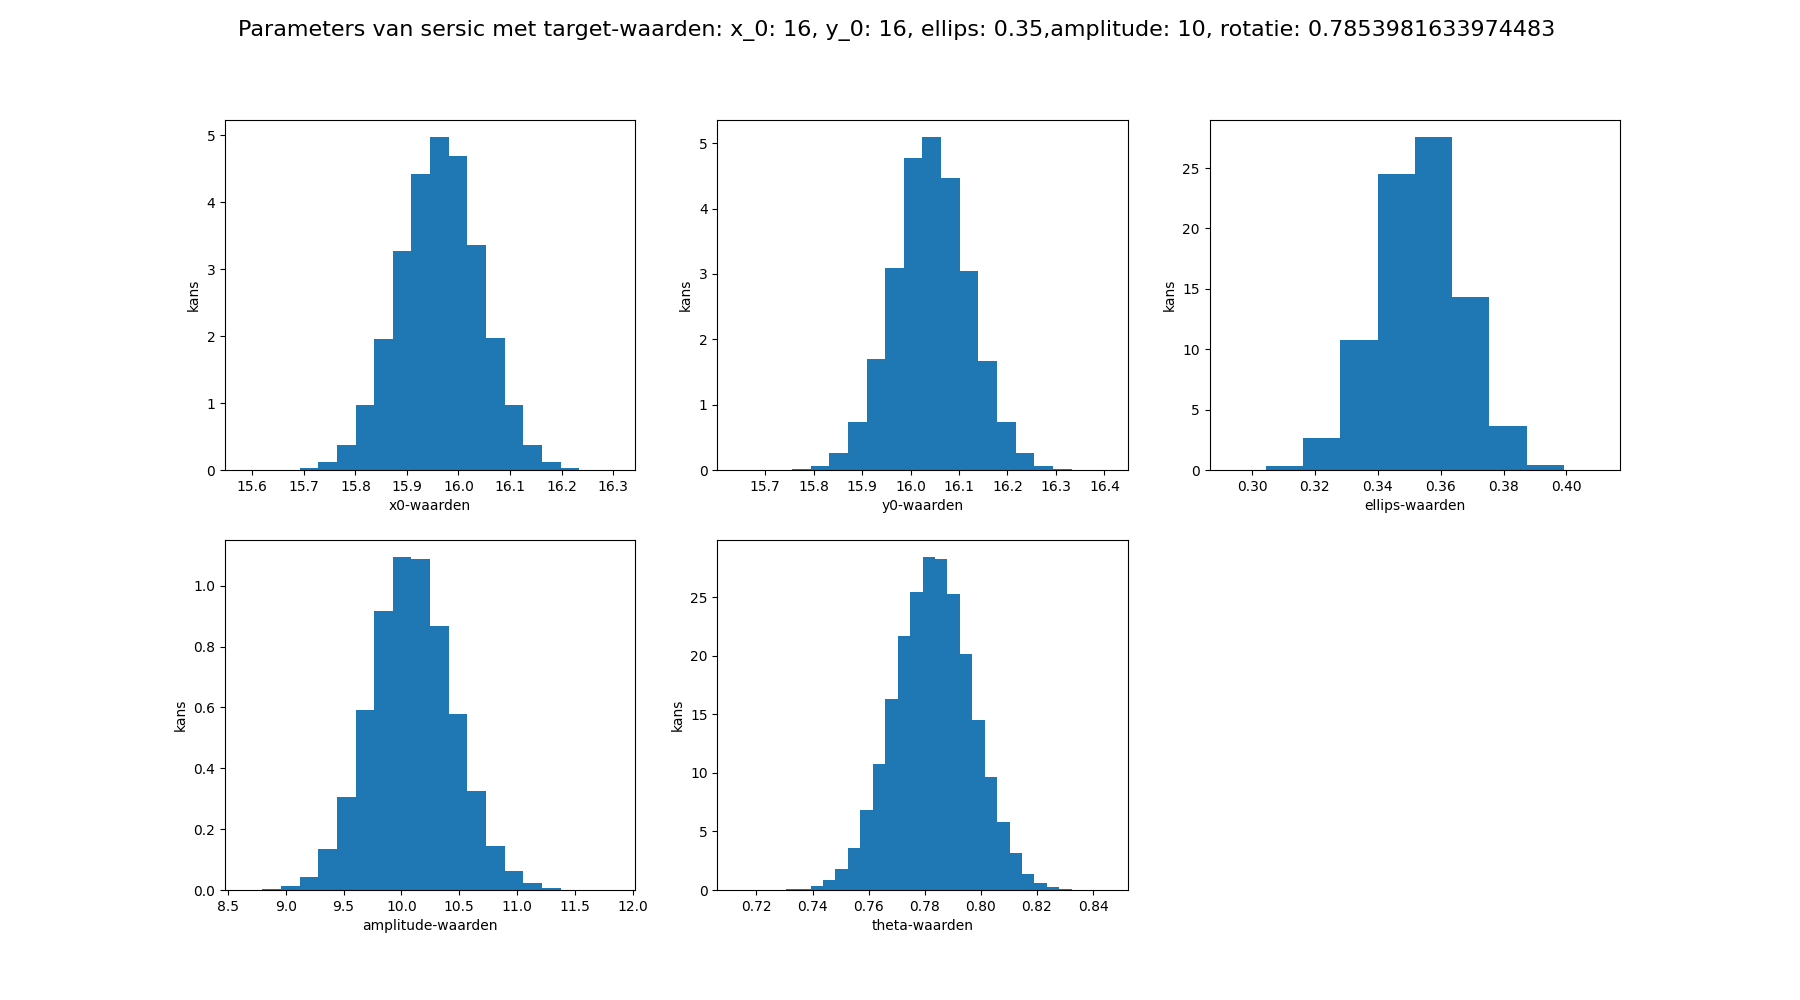
\includegraphics[width=0.93\textwidth]{Figures/1_sersic_verschillende_parameters/sersic_parameters_metropolis_7500000_1500000_10_theta.png}
        \subcaption{5 onbekende parameters}
    \end{minipage}
    \caption{Het proces waarin telkens meer onbekende toegevoegd worden. Er wordt begonnen met vier ongekende parameters, en toegewerkt naar vijf onbekenden.}
    \label{fig:4 onbekenden}
\end{figure}
\begin{figure}
    \centering        
    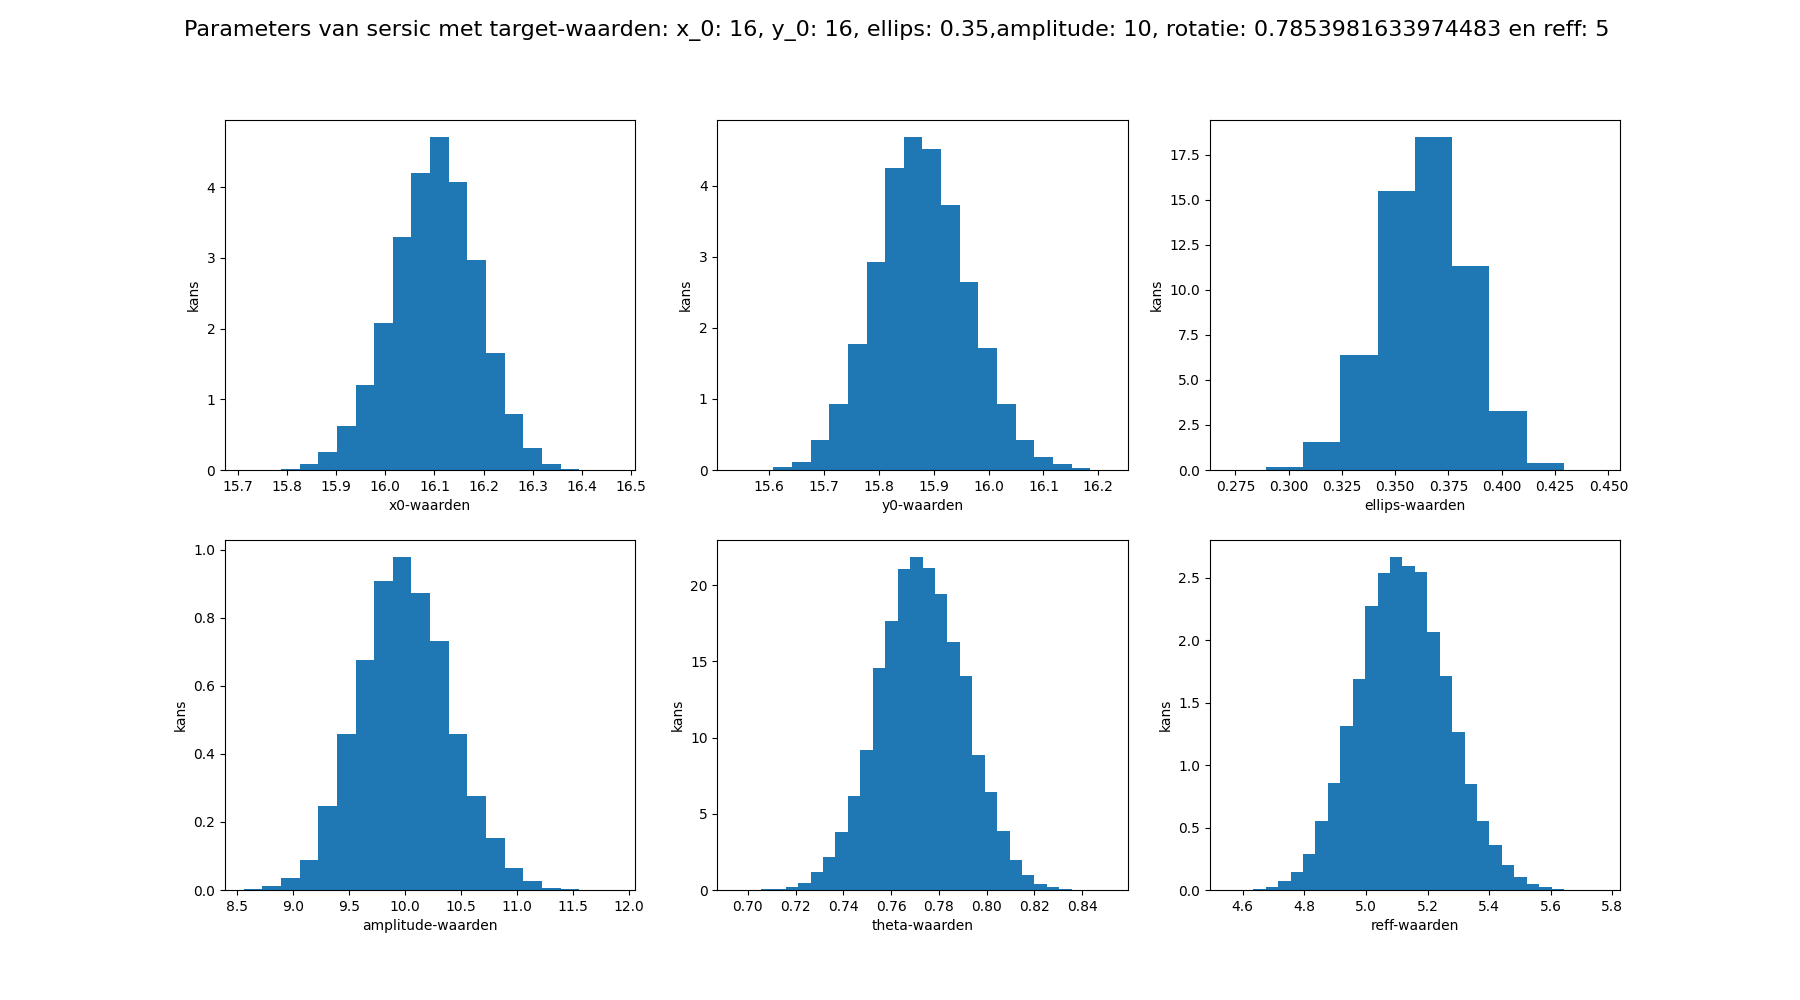
\includegraphics[width=0.93\textwidth]{Figures/1_sersic_verschillende_parameters/sersic_parameters_metropolis_7500000_1500000_10_reff_0.png}
    \caption{Het resultaat van het proces, waarin er zes onbekende parameters afgeschat worden.}
    \label{fig:6 onbekenden}
\end{figure}
\newpage
\twocolumn